\documentclass[10pt]{article}
\usepackage[margin=0.68in]{geometry}
\usepackage[T1]{fontenc}
\usepackage{lmodern}
\usepackage{microtype}
\usepackage{graphicx}
\usepackage{booktabs}
\usepackage{tabularx}
\usepackage{array}
\usepackage{amsmath}
\usepackage{xcolor}
\usepackage{enumitem}
\usepackage{xurl}
\usepackage{hyperref}
\usepackage{caption}
\usepackage{placeins}
\hypersetup{colorlinks=true,linkcolor=blue!55!black,urlcolor=blue!55!black,citecolor=blue!55!black}
\graphicspath{{figures/}}
\setlength{\parskip}{0.30em}
\setlength{\parindent}{0pt}
\setlength{\emergencystretch}{1em}
\renewcommand{\arraystretch}{1.04}
\captionsetup{font=small,labelfont=bf}
\setlist{nosep,leftmargin=*}
\newcommand{\pp}{\ensuremath{\,\mathrm{pp}}}
\newcommand{\ci}[2]{[#1,\,#2]}
\newcolumntype{Y}{>{\raggedright\arraybackslash}X}

\title{Same-Challenge Retrieval in Human and Agent CTF Logs:\\A Paired Measurement Study}
\author{AttackAgent Detect Research}
\date{6 November 2026}

\begin{document}
\maketitle

\begin{abstract}
Security teams may need to retrieve related traces from mixed Human and Agent logs, but a shared benchmark task is only a retrieval proxy, not evidence of a shared operator or attack. We measure how recorded role composition changes same-challenge retrieval errors and whether local-behavior/sequence features (B/S) add information beyond command evidence. In 17 Cyber Task Horizons (CTH) tasks, increasing the Agent share from 0\% to 100\% changes the action-bigram baseline's false-merge rate from 32.27\% to 9.18\% and false-split rate from 52.94\% to 97.87\%. Hit@1 is nearly unchanged (53.13\% to 53.08\%), while gallery AUC falls 11.48 points; the thresholded error shift therefore does not mean that candidate order improves. The primary matched analysis finds no common B/S gain. An exploratory XGBoost diagnostic with expanded training-pair coverage and value-redacted command-argument syntax yields a conditional +6.25-point balanced-accuracy increment (nominal 95\% CI [+1.17,+12.24]), but its max-T interval across four related contrasts includes zero ([-0.75,+13.24]). Agent-only CTH and NYU evaluations also show opposing B/S error trade-offs. The evidence supports reporting composition, ranking, and both error rates separately; it does not support a general behavioral-fingerprint claim.
\end{abstract}

\section{Introduction}
Event-correlation systems use temporal, provenance, causal, or technique evidence to connect records into investigation narratives~\cite{holmes,poirot,atlas,ostinato}. Security datasets increasingly include command traces from both human participants and tool-using Agents~\cite{cth,tang,nyu,ait}. Analysts may want to find logs that merit joint review. A common benchmark label, however, can only test whether traces concern the same challenge. It does not establish a common activity, campaign, actor, or Agent instance.

This distinction matters because two records can share a challenge while following different paths, and two runs can look alike because the collection interface or command adapter makes them alike. Prior Agent-trace work studies model or harness identification, trajectory representation, and synthetic campaign links~\cite{trace,lidar,procgrep,crossagent}. Those tasks are related, but do not measure same-challenge retrieval under changing Human/Agent gallery composition. We ask: (RQ1) how does recorded role composition change ranking and fixed-threshold errors on the same tasks and candidates? (RQ2) does a local behavior and sequence fingerprint add retrieval value beyond command evidence when candidate pairs are held fixed?

We report a controlled CTH role-mixture measurement, a fixed control for log volume and sequence order, and two frozen Agent-only task confirmations. CTH records Human terminal inputs and Agent tool calls through different interfaces; its original collection does not establish that Human participants never used AI~\cite{cthstudy}. Therefore, the mixture is an observed-record composition contrast, not a causal estimate of execution mode.

\section{Representation and evaluation}
\paragraph{Feature design.} The 24-column window schema is a candidate measurement taxonomy with eight slots per block, not a feature count derived from theory or selected against the same-task labels. Prior computer-security user models treated command order and inter-command timing as complementary behavior signals; UNIX profiling also considered command execution time~\cite{mcmahon,dao}. This supports timing as a plausible feature family, but not these particular eight summaries or their value for same-challenge retrieval. Earlier work found timing less promising than command-string evidence, so we treat the timing block as exploratory. T1--T6 summarize launch gaps; T7--T8 are optional duration-derived extensions. In the 24-slot schema, CTH and NYU have no timing fields in the normalized traces used here, while AIT provides process-launch timestamps for T1--T6 but no event durations for T7--T8. The AIT implementation retains the two all-missing slots as constants after fold imputation; only six T measures carry observed variation. CTH and NYU therefore use 16 B/S measurements per window. With a four-event window and mean/standard-deviation pooling, each B and S block contributes 16 pairwise differences; with mean, standard deviation, and trend pooling each contributes 24. CTH's original outer folds selected both pooling/fusion settings, while the two Agent-only confirmations use the frozen four-event, mean/standard-deviation, command-conditioned B/S configuration.

The evidence arm, E, contains command TF--IDF cosine and action-bigram TF--IDF cosine. B/S is appended as the absolute difference between training-standardized trace summaries, using the fold-selected direct or command-conditioned fusion. Where a required block is wholly unavailable for a pair, the frozen E score and threshold are used. No task, role, source, path, tool output, or challenge text is a model input.

\paragraph{Cohorts and protocols.} Table~\ref{tab:protocols} separates the mixed-role measurement from the two Agent-only confirmations. All labels indicate same-task/challenge retrieval. CTH's 17-task mixture cohort requires at least two Human and two Agent traces per task. Its 170 paired allocations assign exactly 0, 25, 50, 75, or 100\% Agent roles to 32 query/candidate slots; each gallery has one same-task and three different-task candidates. The same tasks, draws, and candidates recur across shares. We use the existing command and action-bigram baselines and the frozen three-fold CTH pair predictions.

\begin{table}[!ht]
\centering\footnotesize
\caption{Evaluation cohorts and their distinct fitting protocols. Pair counts are per model arm.}
\label{tab:protocols}
\begin{tabularx}{\linewidth}{@{}p{.17\linewidth}p{.14\linewidth}p{.12\linewidth}p{.35\linewidth}Y@{}}
\toprule
Cohort & Tasks / traces & Pairs & Training and threshold & Role coverage \\
\midrule
CTH mixture & 17 / 85 & 54,400 & Task-held-out CTH; training-only representation/parameter selection and OOF threshold & Mixed; five paired shares \\
CTH AA & 26 / 59 & 23,600 & 17 CTH tasks; 272 sampled pairs; OOF threshold at FMR $\leq10\%$ & Agent--Agent \\
NYU D-CIPHER & 160 / 585 & 234,000 & 17 CTH tasks; 3,570 weighted pairs; OOF threshold at FMR $\leq10\%$ & Agent--Agent \\
AIT logs & 12 / 109 & 43,600 & Task-held-out AIT folds; T1--T6 launch gaps only; no T7--T8 durations & Human and Agent \\
\bottomrule
\end{tabularx}
\end{table}

The CTH timing entries describe the normalized views used here, not all metadata in the upstream archive. Its raw Human logs contain terminal I/O timing, while Agent logs use timestamped Inspect events; we have not validated a shared per-command start/end mapping and do not treat the archive as a comparable timing test in this paper~\cite{cth,inspect}.

The CTH AA confirmation contains new CTH task groups, while NYU uses four public D-CIPHER submission snapshots and challenge slugs excluded from CTH development. The two confirmation sets differ in training-pair construction: sampled pairs for CTH AA and all eligible pairs with label/pair-type balancing weights for NYU. Their difference cannot be attributed to source. The NYU threshold is transferred from CTH and is not expected to preserve the validation FMR on the test source~\cite{nyu}.

\paragraph{Outcomes and uncertainty.} False-merge rate (FMR) is the fraction of different-task pairs accepted; false-split rate (FSR) is the fraction of same-task pairs rejected; $\mathrm{BA}=1-(\mathrm{FMR}+\mathrm{FSR})/2$. For CTH, rates are first averaged within task, then equally over tasks and the five shares. Hit@1 and gallery AUC compare the one positive against three negatives within each query gallery. Intervals use 10,000 paired bootstrap draws of query-task clusters. Repeated galleries and pair rows are not independent, and because candidate tasks recur across query galleries, this bootstrap does not capture all dependence. The original CTH 10\% FMR rule is an inner validation constraint, not a guarantee on held-out tasks or external sources.

\section{Results}
\subsection{Composition moves threshold errors; ranking does not improve}
Figure~\ref{fig:mixture} separates action-bigram ranking from its fixed-threshold decisions. From all-Human to all-Agent role allocations, FMR falls 23.09 points (95\% paired task interval $[-39.88,-8.36]$), while FSR rises 44.93 points ([+21.40,+68.46]); BA falls 10.92 points ([-20.56,-2.90]). Hit@1 changes by $-0.05$ points ([-12.96,+12.91]) and gallery AUC by $-11.48$ ([-25.29,+3.83]). Thus the prominent change is a shift in which class crosses the frozen threshold, alongside uncertain deterioration in score separation; it is not a gain in candidate ranking.

\begin{figure}[!ht]
\centering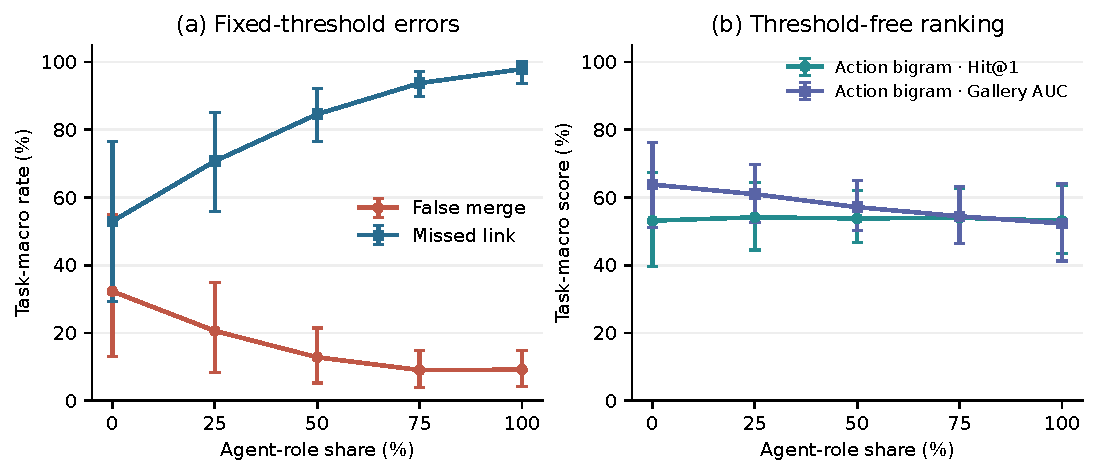
\includegraphics[width=.98\linewidth]{mixture-ranking-shortpaper.pdf}
\caption{Action-bigram cosine across the five paired CTH role shares. Left: task-macro FMR and FSR at the historical fixed threshold. Right: threshold-free Hit@1 and gallery AUC. Error bars are 95\% task-cluster bootstrap intervals. Role share is the allocated query/candidate slots, not the proportion of all source traces.}
\label{fig:mixture}
\end{figure}

Leave-one-task-out analysis preserved the FMR decrease in all 17 omissions and the FSR increase in all 17. A stricter sequence-overlap audit found 30 held-out traces whose full normalized command-head sequence appeared in the corresponding CTH training fold (9/30, 5/30, and 16/25 by fold). Removing every complete gallery containing one of those traces retained 2,114 of 13,600 galleries and 15 query tasks overall; only five tasks remained at both endpoint shares. In that small subset the action-bigram FMR endpoint difference was zero and FSR increased 20 points, with wide intervals. The full-cohort pattern is therefore a paired measurement result under the original task split, not a sequence-disjoint replication.

\subsection{B/S does not add a stable gain beyond simple controls}
The original matched CTH XGBoost comparison gives $\Delta$BA $=-2.38$ points (95\% interval $[-7.29,+2.30]$), with FMR $+9.46$ and FSR $-4.70$ points. The mechanism control holds the 54,400 galleries, three folds, XGBoost depths, and each fold's selected B/S representation fixed. At the equally weighted five-share mean, adding recognized-command and raw-chunk counts to E changes BA by $-3.04$ points. Adding normalized command LCS to that control decreases FMR by 3.21 points ([-5.28,-1.35]) but changes BA by only $+0.54$ ([-3.55,+4.73]), Hit@1 by $-0.05$ ([-1.47,+1.24]), and AUC by $-0.81$ ([-2.78,+0.94]).

Adding real B/S to the same count control changes BA by $-0.79$ points ([-4.96,+3.51]), Hit@1 by $-0.93$ ([-5.09,+3.30]), and gallery AUC by $-0.84$ ([-6.78,+5.04]). None of the five predeclared shuffled-order seeds yields an interval excluding zero for these three outcomes when compared with real B/S at the equal-share mean. The primary matched experiment therefore does not isolate a common B/S increment beyond trace volume and command evidence. A separate development diagnostic varies training-pair coverage and adds value-redacted command-argument syntax to the evidence baseline. Under all-pair training, XGBoost E+Args+B/S improves BA over E+Args by $6.25$ points (nominal 95\% task interval [+1.17,+12.24]), with FSR down 13.06 and FMR up 0.56 points. The max-T interval across the four examined coverage-by-baseline contrasts is [-0.75,+13.24], so this is a conditional signal for follow-up, not a confirmed or learner-common gain (Supplement, Section~\ref{sec:pairsupport}).

\subsection{Agent-only confirmations show different error trade-offs}
Table~\ref{tab:external} reports the XGBoost absolute rates and paired changes. CTH AA reduces false merges but increases false splits, yielding an uncertain BA decline. NYU does the reverse, with a BA gain, but its B/S arm's FMR is 25.39\% despite CTH calibration at 10\%. NYU XGBoost also gains 3.20 points in Hit@1 ([+0.51,+5.92]) and 2.07 in candidate-pair AP ([+0.04,+4.08]); its gallery-AUC change is uncertain at +1.82 ([-0.38,+3.97]). SVM loses 8.23 BA points, and the decision tree's BA gain accompanies lower ranking metrics. These panels do not establish a common B/S effect across learners or sources.

\begin{table}[!ht]
\centering\scriptsize
\caption{Frozen XGBoost comparisons. Rates are task-macro percentages. Changes are E+B/S minus E, in percentage points; intervals are paired task-cluster 95\% intervals.}
\label{tab:external}
\setlength{\tabcolsep}{2pt}
\begin{tabularx}{\linewidth}{@{}p{.12\linewidth}p{.16\linewidth}p{.16\linewidth}p{.17\linewidth}p{.17\linewidth}Y@{}}
\toprule
Evaluation & E FMR / FSR & E+B/S FMR / FSR & $\Delta$FMR & $\Delta$FSR & $\Delta$BA \\
\midrule
CTH mixture & 5.97 / 81.91 & 15.43 / 77.21 & +9.46 [5.50, 13.74] & $-4.70$ [$-15.45$, 6.10] & $-2.38$ [$-7.29$, 2.30] \\
CTH AA & 11.78 / 78.04 & 5.63 / 91.06 & $-6.14$ [$-9.96$, $-2.37$] & +13.03 [2.71, 25.67] & $-3.44$ [$-9.71$, 1.93] \\
NYU AA & 10.72 / 86.96 & 25.39 / 60.86 & +14.67 [13.28, 16.06] & $-26.10$ [$-30.72$, $-21.38$] & +5.71 [3.63, 7.73] \\
\bottomrule
\end{tabularx}
\end{table}

\section{Discussion and conclusion}
The main finding is an operating-point sensitivity: when the recorded role assigned to fixed CTH task galleries changes, a frozen action-similarity threshold shifts from accepting many different-task pairs to rejecting nearly all same-task pairs. Hit@1 barely changes and gallery AUC trends down. This distinction matters for analyst triage, where ranking can prioritize candidates, and for automatic linking, where a transferred threshold controls false merges. In a three-negative no-match stress check, 39.49\% of all-Agent CTH galleries using the frozen B/S XGBoost arm accept at least one negative; the corresponding E rate is 20.63\%. The threshold's validation target alone would hide this gallery-level burden.

The mechanism analysis offers a more specific answer about feature provenance. Local B/S measurements are interpretable summaries of observed traces, but their count and apparent coverage do not guarantee task-retrieval value. A simple command-subsequence similarity changes the false-merge operating point. The primary matched control does not show a common B/S gain, while an exploratory XGBoost result suggests B/S may add recall-side value after training coverage expands and command argument syntax is already represented; its simultaneous interval remains compatible with no gain. The 24-window-column taxonomy should therefore be treated as a measurement schema, not as 24 validated association predictors. Existing nested deletion results also select different single-feature removals across folds and do not justify pruning a stable subset.

Three limitations bound the result. First, only 17 mixed-role CTH tasks support the composition study, and task-disjoint folds still share some exact command sequences across training and held-out tasks. Second, collection interface and recorded role covary, so the mixture is not causal evidence about human versus Agent execution. Third, CTH AA and NYU AA differ in training-pair construction, while NYU covers four D-CIPHER snapshots within one framework; neither supplies independent mixed-role confirmation. The benchmark label remains same-task identity throughout.

We conclude that any claim about trace fingerprints should report the target relation, role composition, score ranking, both error rates, and threshold transfer together. Composition-related error migration is the clearest result; the strongest same-task B/S result is conditional on one learner, expanded pair coverage, and a richer command baseline, and still needs independent replication. The practical result is a measurement caution for same-challenge retrieval, not an attribution capability.

\begin{thebibliography}{99}\footnotesize
\bibitem{trace} M. Ediga and S. Chattopadhyay. Trace: Unmasking AI Attack Agents Through Terminal Behavior Fingerprinting. arXiv:2605.01186, 2026. \url{https://arxiv.org/abs/2605.01186}
\bibitem{procgrep} H. Oderinwale. Agent Trajectories as Programs: Fingerprinting and Programming Coding-Agent Behavior. arXiv:2606.16988, 2026. \url{https://arxiv.org/abs/2606.16988}
\bibitem{lidar} C. Wang et al. Who Is Behind the Harness? Fingerprinting LLMs through Agentic Behavior. arXiv:2609.28559, 2026. \url{https://arxiv.org/abs/2609.28559}
\bibitem{crossagent} S. Park et al. Cross-Agent Campaign Attribution: Linking Asynchronous Attacks Across LLM Agents. arXiv:2607.18826, 2026. \url{https://arxiv.org/abs/2607.18826}
\bibitem{tang} T. Tang et al. From Assistance to Autonomy: An Empirical Study of AI Use in a Live Capture-the-Flag (CTF) Competition. 35th USENIX Security Symposium, 2026, pp. 6645--6664. \url{https://www.usenix.org/conference/usenixsecurity26/presentation/tang-tingxuan}
\bibitem{cth} Lyptus Research. Cyber Task Horizons Data. Dataset and collection report, 2026. \url{https://github.com/lyptus-research/cyber-task-horizons-data}
\bibitem{mcmahon} M. M. McMahon and H. A. Sholl. Influence of State Size on User Models in a Network Security System. 13th International Conference on Parallel and Distributed Computing Systems, 2000. \url{https://www.researchgate.net/publication/282647993_Influence_of_State_Size_on_User_Models_in_a_Network_Security_System}
\bibitem{dao} V. N. P. Dao, R. Vemuri, and S. J. Templeton. Profiling Users in the UNIX OS Environment. Lawrence Livermore National Laboratory preprint UCRL-JC-141022, 2000. \url{https://www.osti.gov/servlets/purl/15004770}
\bibitem{inspect} UK AI Safety Institute. Inspect AI: Event Reference. \url{https://inspect.aisi.org.uk/reference/inspect_ai.event.html}
\bibitem{cthstudy} Lyptus Research. Cyber Task Horizons: Human Evaluation Setup. \url{https://lyptusresearch.org/research/offensive-cyber-time-horizons#human-evaluation-setup}
\bibitem{nyu} NYU-LLM-CTF. Leaderboard Submissions. GitHub repository, revision recorded in the frozen manifest. \url{https://github.com/NYU-LLM-CTF/leaderboard_submissions}
\bibitem{ait} AIT Austrian Institute of Technology. LLM User Shell Simulation. GitHub repository. \url{https://github.com/ait-aecid/llm-user-shell-sim}
\bibitem{atlas} A. Alsaheel et al. ATLAS: A Sequence-Based Learning Approach for Attack Investigation. USENIX Security Symposium, 2021. \url{https://www.usenix.org/conference/usenixsecurity21/presentation/alsaheel}
\bibitem{holmes} M. Milajerdi et al. HOLMES: Real-Time APT Detection through Correlation of Suspicious Information Flows. IEEE S\&P, 2019. \url{https://arxiv.org/abs/1810.01594}
\bibitem{ostinato} S. K. Ghosh et al. OSTINATO: Cross-Host Attack Correlation through Attack Activity Similarity Detection. arXiv:2312.09321, 2023. \url{https://arxiv.org/abs/2312.09321}
\bibitem{poirot} S. M. Milajerdi et al. POIROT: Aligning Attack Behavior with Kernel Audit Records for Cyber Threat Hunting. ACM CCS, 2019. \url{https://arxiv.org/abs/1910.00056}
\end{thebibliography}
\end{document}
